
\documentclass[a4paper, 12pt, onecolumn, oneside]{report}

\usepackage{geometry} 
\geometry{a4paper} 
\usepackage{graphicx} 
\usepackage{float}
\usepackage{wrapfig} 
\usepackage{lipsum} 
\usepackage  [utf8] {inputenc}
\usepackage  [portuguese] {babel}
\linespread{1.2}
%\setlength\parindent{0pt} 
\graphicspath{{./Imagens/}} 
\usepackage{graphicx}
\begin{document}
\begin{titlepage}

\newcommand{\HRule}{\rule{\linewidth}{0.4mm}} % 

\center 


\begin{figure}[H] 
\center{
\includegraphics[width=1.0\linewidth]{UA1}}
\end{figure}


\textsc{\ Departamento de Electrónica, Telecomunicações e Informática
 }\\[0.9cm] 

{\raggedright \textbf{Curso:} [8240] Mestrado Integrado em Eng. de Computadores e Telemática

\textbf{Disciplina:} [47137] Introdução à Eng. de Computadores e Telemática

\textbf{Ano lectivo:} 2012/2013 \\[1cm] 

}


\HRule \\[0.1cm]
{ \huge \bfseries Relatório da Aula Prática 8 \\
[0.4cm]  
Programação do Robô \\ [0.4cm] DETI PIC }\\[0.4cm] 
\HRule \\[1cm]


\begin{minipage}{0.4\textwidth} 
\begin{flushleft} \large
\emph{Autores:}\\
{[68535] Bruno \textsc{Silva}} \\
{[68799] Rui \textsc{Oliveira} } 


\emph{Turma/Grupo:}\\
T5B / Prática 3\\

\end{flushleft}
\end{minipage}
~
\begin{minipage}{0.4\textwidth}
\begin{flushright} \large
\emph{Docentes:} \\
André \textsc{Zúquete} \\
João \textsc{Barraca} \\
\emph{Data:} \\
\today 
\end{flushright}
\end{minipage}\\[2cm]



\vfill 

\end{titlepage}



\vspace*{\fill}



\textbf{Resumo:}


\begin{flushleft}

 Pretende-se através deste relatório expor sob forma escrita, o nosso desempenho e objetivos alcançados na aula de Introdução à Engenharia de Computadores e Telemática. De modo a responder ao protocolo que nos foi estabelecido, programámos o robô DETI PIC, desenvolvido pelo Departamento de Eletrónica, Telecomunicações e Informática da Universidade de Aveiro, e com isso tentar de forma satisfatória atingir os objetivos principais do mesmo.

\end{flushleft}


\vspace*{\fill}

\newpage




\newpage

\renewcommand*\contentsname{Índice}

\tableofcontents 


\newpage
 
\section{Introdução} 


Como sabemos, um robô é um dispositivo, ou conjunto de dispositivos, eletromecânicos ou biomecânicos capazes de realizar uma determinada funcionalidade de forma independente, para isso terá de ser pré-programado, ou então controlado por um ser humano. Primordialmente os robôs foram programados para desenvolver trabalhos de baixa complexidade, como por exemplo, deslocarem-se sobre superfícies planas, interagir com obstáculos, entre outros. Atualmente, os robôs realizam tarefas muito completas, e em muitos dos casos substituindo o trabalho humano. Embora, nem sempre se tira partido de todas as capacidades do robô.

Neste relatório pretendemos demonstrar o nosso desempenho na programação do robô DETI PIC, desenvolvido pelo Departamento de Eletrónica, Telecomunicações e Informática da Universidade de Aveiro. Mais à frente iremos mostrar as principais características do robô, e alguns dos equipamentos e materiais que utilizámos para conseguir concretizar esta actividade. Para a programação de robô utilizando um software, também este desenvolvido pelo DETI, chamado \emph{DETInchanting} criado a partir de linguagem JAVA e C++ e adaptado do \emph{Enchanting}, desenvolvido para robôs da LEGO\footnote{Empresa conceituada no fabrico de brinquedos, e atualmente no desenvolvimento de robôs. }. Neste caso, necessitámos de ter conhecimentos básicos de programação em JAVA, para conseguir testar as capacidades do robô, através da implementação blocos que permitem executar operações do tipo: \emph{if}... \emph{else}...; \emph{forever}... ; \emph{repeat until}... ; entre outros. 

Ambicionamos com estes testes ao robô, explorar os sensores de distância, tentar fazer com que este siga uma parede de modo a contorná-la, e também de conjugar o seguimento de uma parede com a deteção de linhas de cor preta localizadas, neste caso no tampo da mesa. 



\newpage
\section{Descrição do problema}

Pretendemos através deste relatório dar resposta, programando e observando o comportamento do robô DETI PIC de modo a solucionar os seguintes problemas apresentados: 

\begin{itemize}
  \item \textbf{PROBLEMA 1} - Programar o robô de forma a ele deslocar-se em frente até encontrar um obstáculo frontal a menos de 10 cm. Quando tal acontecer, o robô deverá parar e rodar sobre si mesmo, num qualquer sentido de rotação, até que essa distância aumente. Quando tal acontecer, o robô deverá continuar o seu movimento para diante. 
\end{itemize}

\begin{itemize}
  \item \textbf{PROBLEMA 2} - Programar o robô de modo a que este siga uma parede, sempre com o mesmo lado voltado para a parede, sem nunca lhe tocar.
\end{itemize}

\begin{itemize}
  \item \textbf{PROBLEMA 3} - Alterar o programa anterior para detetar a presença de linhas pretas nos chãos perpendiculares à parede. Sempre que as detetar deverá parar durante algum tempo e sinalizar a sua deteção com os leds, após o que deve retomar o movimento anterior. 
\end{itemize}

\begin{itemize}
  \item \textbf{PROBLEMA 4} - Altere o programa anterior para inverter o sentido de deslocamento sempre que encontrar uma linha preta perpendicular a uma parede, devendo a partir desso ponto seguir a parede mantendo o outro lado voltado para a mesma. 
\end{itemize}


Para além dos quatro problemas acima descritos, pretendemos também adquirir alguns dos conhecimentos introdutórios do funcionamento e programação da robótica utilizando para isso o \emph{DETInchanting}, programa este que iremos abordar mais à frente. Dado que nos foi imposto a realização deste relatório utilizando a linguagem tipo \LaTeX, pretendemos também desenvolver as nossas competências a nível desta linguagem, alargando assim os nossos conhecimentos já adquiridos em aulas anteriores.   





\newpage
\section{Aparelhagem e equipamento}



\subsection{Robô DETI PIC}

A nossa base de trabalho é o robô DETI PIC. Este robô é constituído por dois motores DC\footnote{Corrente contínua} sem realimentação, três sensores de distância frontais cobrindo um ângulo de aproximadamente 45 graus para cada lado do robô, cinco sensores de brilho na parte inferior do robô e quatro led's na parte superior. O robô dispõe ainda de dois botões, um interruptor e uma porta USB. Todo este robô foi desenvolvido de forma prática e intuitiva à introdução à programação deste tipo de máquinas. 
Para fazer o upload entre o robô e o computador utilizá-mos um cabo USB\footnote{Universal Serial Bus} 2.0.



\begin{figure}[H] 
\center{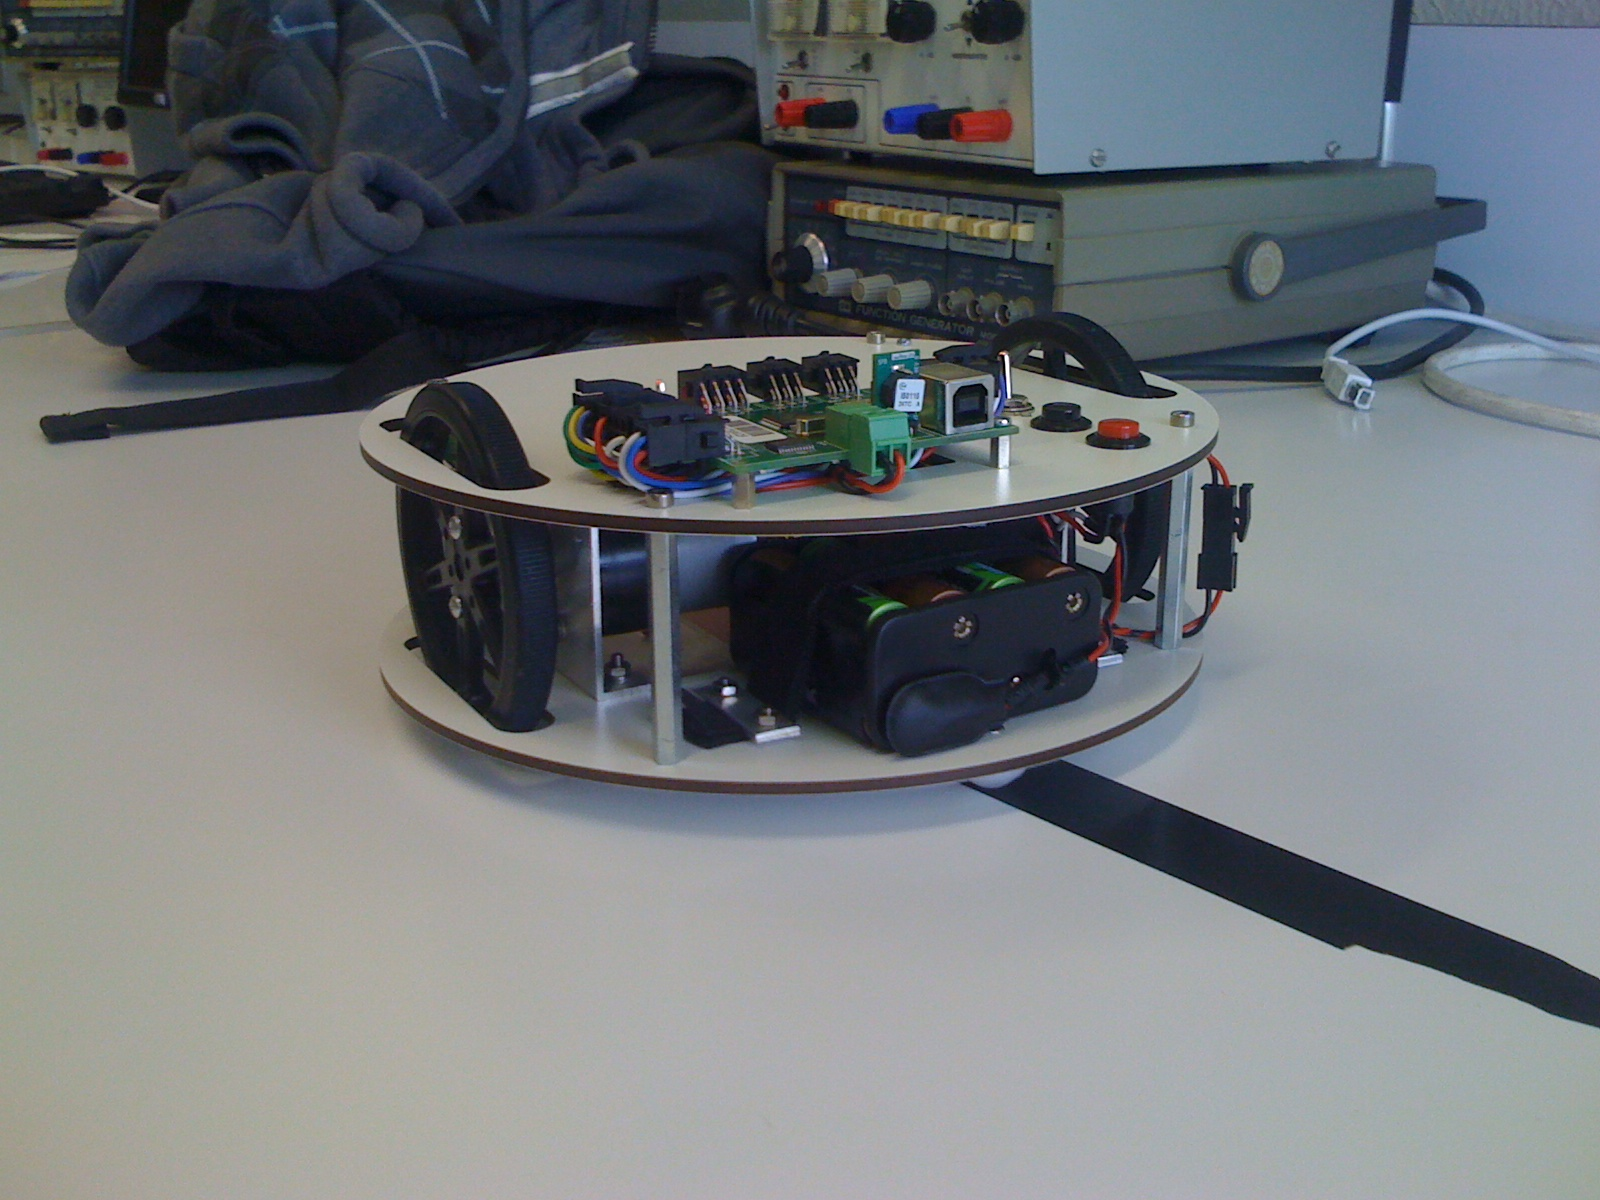
\includegraphics[width=0.5\linewidth]{robo2}}
\caption{Robô DETI PIC}
\label{fig:speciation}
\end{figure}


\subsection{Software DETInchanting}

O programa usado para a programação de instruções a dar ao robô neste trabalho foi o \emph{DETInchanting}, uma adaptação do original \emph{Enchanting} usado para programar robôs da LEGO. Este interface foi desenvolvido na Universidade de Aveiro com a intenção de facilitar a programação dos robôs utilizando um interface gráfico que se baseava em encaixes de blocos de código JAVA, na Figura 2 está representada o ambiente de trabalho deste programa. Este sofware usa um paradigma gráfico do tipo Scratch\footnote{São interfaces gráficos que permitem que programas sejam criado através da sobreposição de blocos, tendo na sua base linguagens de programação.}.



\begin{figure}[H] 
\center{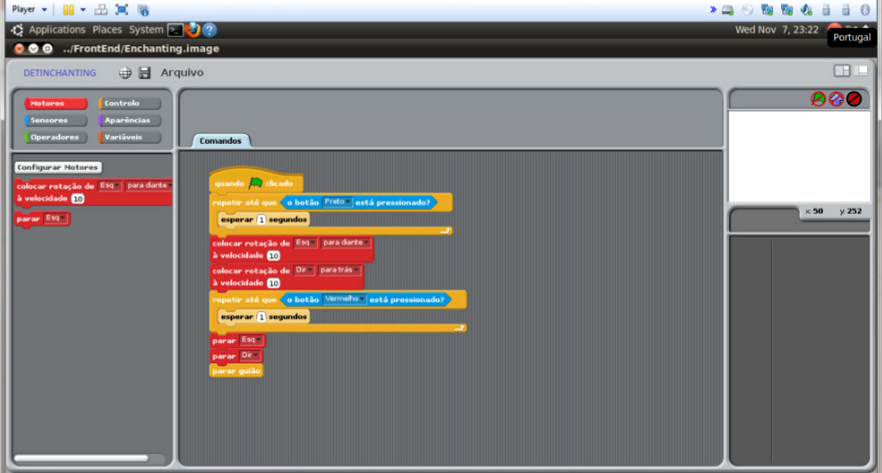
\includegraphics[width=0.9\linewidth]{ambiente}}
\caption{Ambiente do \emph{DETInchanting.}}
\label{fig:speciation}
\end{figure}




\subsection{Materiais utilizados}

O nosso ambiente de trabalho foi a bancada dos laboratórios do DETI o que não nos dava muito espaço para manobrar os robôs. Nestas condições usamos duas folhas A4 com uma linha preta impressa para o robô seguir, e um parede em forma de "L" em K-Line para fazer o robô evitar.






 \newpage
 
\section{Procedimento}

\subsection{Problema 1}

Como dissemos anteriormente o \emph{DETInchanting} funciona à base da implementação de blocos pré-definidos. Dos que estão disponíveis no software iremos utilizámos os que de seguida estão mencionados.

Para inicializar o programa iremos utilizar o bloco “\emph{when clicked}”, de seguida com um ciclo \emph{repeat 
until} ao pressionar o botão \emph{Red} o programa irá mover o robô e o programa inicia-se.

Num ciclo repetitivo \emph{forever}, iremos inserir um ciclo opcional, do tipo \emph{if...else}, neste caso quando os sensores \emph{right}, \emph{front} e \emph{left} não detectarem nenhum obstáculo a mais de 10 cm, os motores (esquerdo e direito) irão mover-se de modo a que o robô se desloque para a frente, caso contrário, ou seja se os sensores encontrarem um obstáculo a menos de 10 cm, o robô irá afastar-se do mesmo. Neste ultimo caso os blocos irão dispor-se dentro de um ciclo \emph{if...else} em que se o sensor \emph{left} encontrar um obstáculo o motor esquerdo irá mover-se para a frente enquanto que o motor direito irá mover-se para trás. Se forem os sensores \emph{front} e \emph{right} a detectar o obstáculo, então o motor esquerdo irá mover-se para trás enquanto que o direito irá mover-se para a frente. Desta forma o robô DETI PIC tentará evitar a parede.

\subsection{Problema 2}

De forma a solucionarmos este problema ,iremos  começar por criar 2 variáveis "dDir" e "dEsq" que representavam a distância direita e esquerda respectivamente. A essas variáveis eram atribuídas os valores da distância medidas pelos sensores do lado direito e esquerdo para uso futuro no programa. O uso destas variáveis reduz significativamente o tempo de execução de um ciclo do programa uma vez que a tarefa que demora mais tempo, que é a leitura do valores lidos pelos sensores, fica reduzido a uma vez por ciclo.

Após a leitura das variáveis o robô vai avaliar essas distâncias e compará-las com valores introziduzidos pelos executantes de forma a que se mantenha a uma distância da parede que não lhe "toque" mas também que não se afaste. Isto é feito através de uma condição \emph{if...else} onde o apresentado anteriormente se encontra no interior da condição \emph{if}. Dentro do \emph{else} encontram-se mais dois \emph{if}'s que servem para fazer as correcções das distâncias. O primeiro corrige a trajectória do robô caso este se encontre muito afastado da parede, e o segundo faz o contrário aproximando o robô da parede caso este se encontre perto de mais. Todos estes passos estão envolvidos por um ciclo \emph{forever} que faz com que este processo seja repetido infinitamente.

 \newpage
\section{Resultados}

\subsection{Problema 1}

Através da implementação e criação do programa apresentado na Figura 3, conseguimos obdecer ao enunciado do Problema 1.

Ao realizarmos o upload do programa que apresentamos de seguida conseguimos com que o nosso robô evitasse a parede e de seguida se afastasse dela. 

\begin{figure}[H]
\center{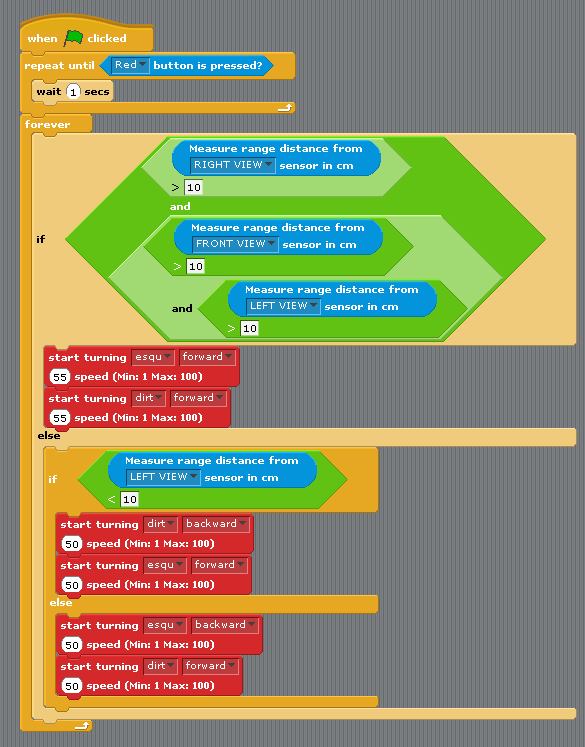
\includegraphics[width=0.7\linewidth]{probl1}}
\caption{Resolução do problema 1 utilizando o software DETInchanting}
\label{fig:speciation}
\end{figure}


\subsection{Problema 2}

Através da implementação e criação do programa apresentado na Figura 3, conseguimos obdecer ao enunciado do Problema 2, embora com algumas limitações que iremos apresentar na próxima secção.



\begin{figure}[H]
\center{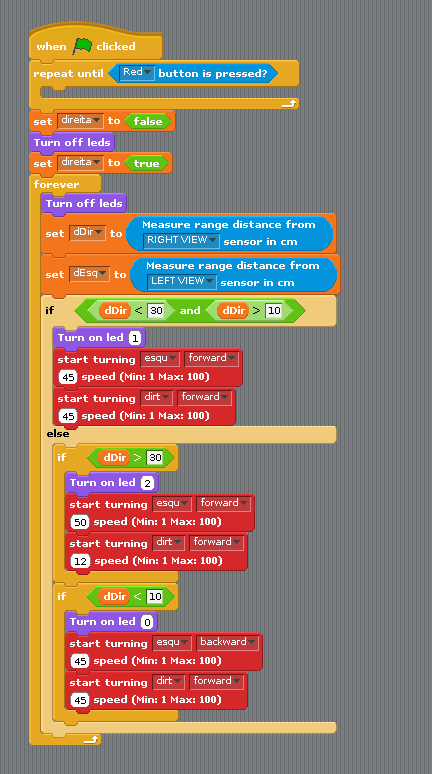
\includegraphics[width=0.5\linewidth]{probl2}}
\caption{Resolução do problema 2 utilizando o software DETInchanting.}
\label{fig:speciation}
\end{figure}






\subsection{Problemas 3 e 4}

Devido à falta de tempo não conseguimos resolver os problemas 3 e 4.






 \newpage
 






\section{Análise dos Resultados}




\subsection{Problema 1}

Tal como pretendíamos o nosso programa funcionou da maneira que esperávamos, ou seja de acordo com o enunciado do problema 1. Na figura 5 está esquematizado o movimento levado a cabo pelo robô, na execução deste algoritmo, representado por uma linha a tracejado.


\begin{figure}[H]
\center{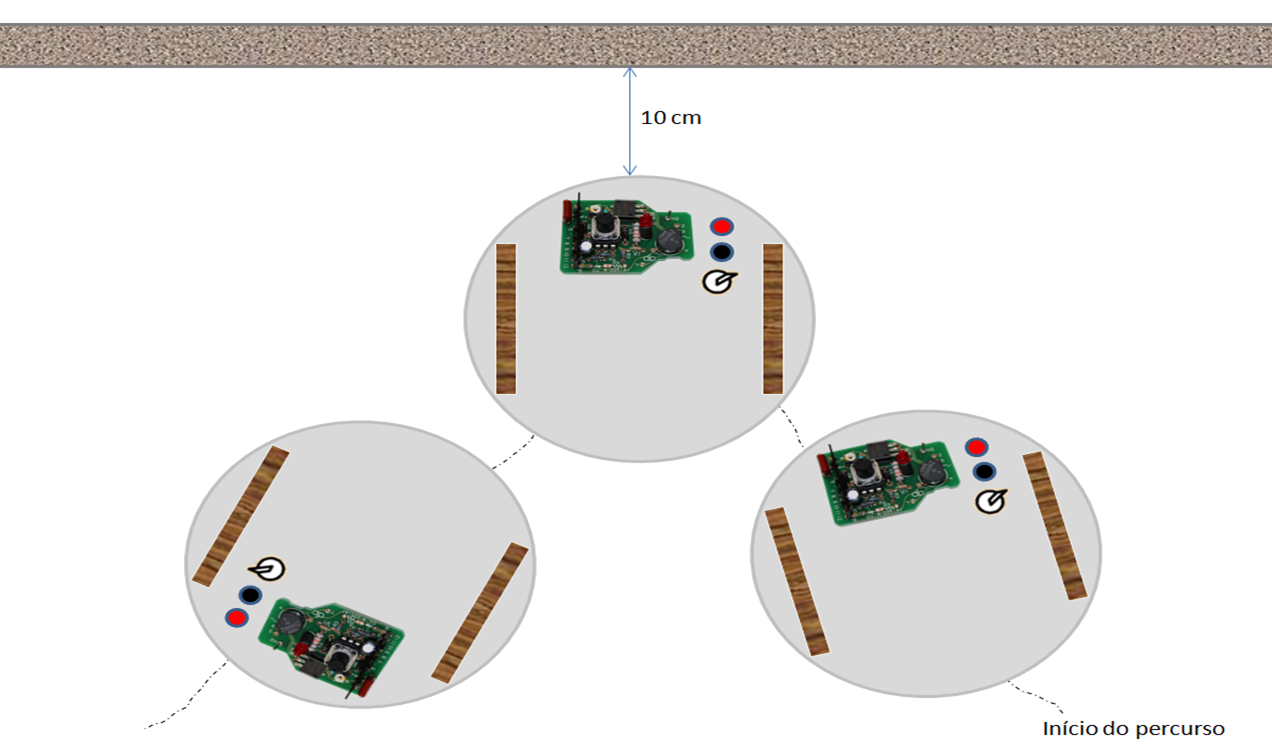
\includegraphics[width=1.0\linewidth]{problema_1}}
\caption{Esquema estroboscópico do problema 1.}
\label{fig:speciation}
\end{figure}

Pensamos que o programa estará a funcionar em perfeitas condições, contudo, poderíamos ter adicionado um bloco que permitisse ao utilizador quando pressionasse o botão \emph{black}, o programa terminaria. Apesar deste pequeno pormenor, consideramos o nosso problema 1, bem-sucedido. 

\newpage

\subsection{Problema 2}
No exercício 2 verificamos alguns problemas ao nível da resolução do algoritmo para o robô executar a tarefa pretendida na perfeição. Embora o robô conseguisse seguir a parede mesmo quando ela não era linear, encontrava problemas quando tinha de "dar a volta" perdendo-se pois "pensava" que era mais uma curva da parede, este trajecto está descrito na Figura 6.  Esse problema incapacitou o robô de efetuar a sua tarefa na totalidade, tornando assim o exercício incompleto.

A solução deste problema poderia ter sido realizada com um pouco mais de tempo. Adicionando mais uma condição ao \emph{if} que corrigia a posição caso se afastasse da parede e assim que limitasse não só a distância mínima (que tomamos como 30) mas também uma máxima (por exemplo 40), assim poderíamos adicionar um \emph{if} em que a condição fosse ">40" em que o robô era programado a contornar a parede.





\begin{figure}[H]
\center{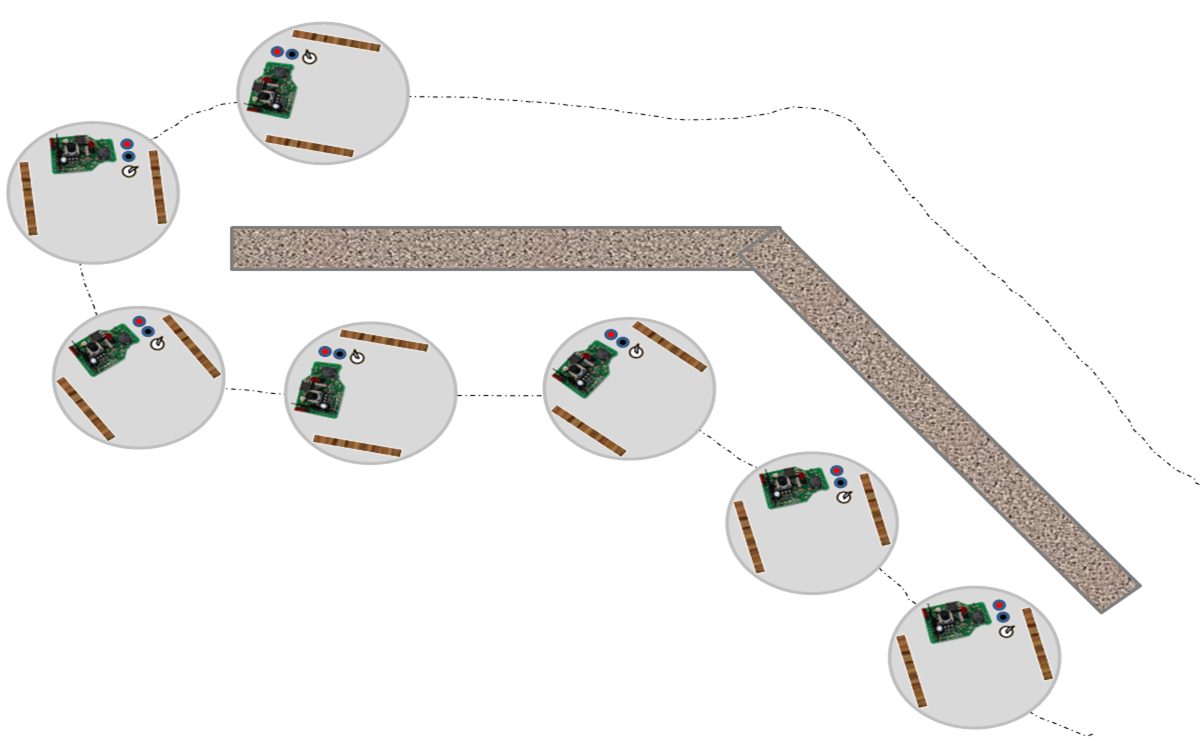
\includegraphics[width=1.0\linewidth]{problema_2}}
\caption{Esquema estroboscópico do problema 2.}
\label{fig:speciation}
\end{figure}





 \newpage

\section{Conclusões}




Chegado ao final deste relatório, é nossa intenção efetuar uma retrospetiva da evolução do mesmo, tendo em conta os problemas que nos deparámos, objetivos, e principais metodologias utilizadas.

Apesar de não termos consigo testar e programar todos os problemas apresentamos na integra, devido ao fator tempo, pensamos que os problemas principais foram bem conseguido, embora o último com algumas dificuldades.


Um dos fatores que também nos poderá ter prejudicado incide ao facto que só tivemos acesso ao problemas para realização a atividade no dia da aula prática, portanto não nos foi possível preparar a atividade antecipadamente como pretendíamos, de modo a termos a totalidade dos programas construídos, prontos a serem testados nos robôs, tal como nos foi sugerido.

Esperamos em problemas futuros conseguir suceder de forma mais eficiente neste âmbito e conseguir um melhor aproveitamento à disciplina. 



\begin{thebibliography}{99} 

\bibitem[1]{Figueredo:2009dg}
A.V.C.M. Zúquete , Site da Unidade Curicular - Introdução à Engenharia de Computadores e Telemática (1 Dezembro 2012).
\newblock Diapositivos: robô DETI PIC [Online]
\newblock {\em Available: } http://www.ieeta.pt/~avz/Aulas/IECT/12-13/docs/6-robo.pdf 

\bibitem[2]{Figueredo:2009dg}
J. Barraca, D. Gomes, A. Zúquete , Site da Unidade Curicular - Introdução à  Engenharia de Computadores e Telemática (1 Dezembro 2012).
\newblock Guião da aula prática 8 [Online]
\newblock {\em Available: } http://www.ieeta.pt/~avz/Aulas/IECT/12-13/docs/guiao-8.pdf 

 
\end{thebibliography}


\end{document}
